\documentclass[letterpaper, 10pt, conference]{ieeeconf}
\IEEEoverridecommandlockouts \overrideIEEEmargins
\usepackage{amsmath,amssymb,url}
\usepackage{graphicx,subfigure,tikz,graphicx}
\usepackage{color}
\newcommand{\argmax}{\operatornamewithlimits{argmax}}

\newcommand{\norm}[1]{\ensuremath{\left\| #1 \right\|}}
\newcommand{\bracket}[1]{\ensuremath{\left[ #1 \right]}}
\newcommand{\braces}[1]{\ensuremath{\left\{ #1 \right\}}}
\newcommand{\parenth}[1]{\ensuremath{\left( #1 \right)}}
\newcommand{\pair}[1]{\ensuremath{\langle #1 \rangle}}
\newcommand{\met}[1]{\ensuremath{\langle\langle #1 \rangle\rangle}}
\newcommand{\refeqn}[1]{(\ref{eqn:#1})}
\newcommand{\reffig}[1]{Fig. \ref{fig:#1}}
\newcommand{\tr}[1]{\mathrm{tr}\ensuremath{\negthickspace\bracket{#1}}}
\newcommand{\trs}[1]{\mathrm{tr}\ensuremath{[#1]}}
\newcommand{\ave}[1]{\mathrm{E}\ensuremath{[#1]}}
\newcommand{\deriv}[2]{\ensuremath{\frac{\partial #1}{\partial #2}}}
\newcommand{\SO}{\ensuremath{\mathsf{SO(3)}}}
\newcommand{\T}{\ensuremath{\mathsf{T}}}
\renewcommand{\L}{\ensuremath{\mathsf{L}}}
\newcommand{\so}{\ensuremath{\mathfrak{so}(3)}}
\newcommand{\SE}{\ensuremath{\mathsf{SE(3)}}}
\newcommand{\se}{\ensuremath{\mathfrak{se}(3)}}
\renewcommand{\Re}{\ensuremath{\mathbb{R}}}
\newcommand{\aSE}[2]{\ensuremath{\begin{bmatrix}#1&#2\\0&1\end{bmatrix}}}
\newcommand{\ase}[2]{\ensuremath{\begin{bmatrix}#1&#2\\0&0\end{bmatrix}}}
\newcommand{\D}{\ensuremath{\mathbf{D}}}
\renewcommand{\d}{\ensuremath{\mathfrak{d}}}
\newcommand{\Sph}{\ensuremath{\mathsf{S}}}
\renewcommand{\S}{\Sph}
\newcommand{\J}{\ensuremath{\mathbf{J}}}
\newcommand{\Ad}{\ensuremath{\mathrm{Ad}}}
\newcommand{\intp}{\ensuremath{\mathbf{i}}}
\newcommand{\extd}{\ensuremath{\mathbf{d}}}
\newcommand{\hor}{\ensuremath{\mathrm{hor}}}
\newcommand{\ver}{\ensuremath{\mathrm{ver}}}
\newcommand{\dyn}{\ensuremath{\mathrm{dyn}}}
\newcommand{\geo}{\ensuremath{\mathrm{geo}}}
\newcommand{\Q}{\ensuremath{\mathsf{Q}}}
\newcommand{\G}{\ensuremath{\mathsf{G}}}
\newcommand{\g}{\ensuremath{\mathfrak{g}}}
\newcommand{\Hess}{\ensuremath{\mathrm{Hess}}}
\newcommand\circled[1]{%
  \tikz[baseline=(C.base)]\node[draw,circle,inner sep=0.5pt](C) {#1};\!
}

\title{\LARGE \bf
%Recursive Kalman-Mahanobis JPDAF Minimization to avoid Coalescence of Estimates in Close Proximity
Optimal Joint Probabilistic Data Association Filter\\ Avoiding Coalescence in Close Proximity }
\author{Evan Kaufman and Taeyoung Lee$^*$
 \thanks{Evan Kaufman and Taeyoung Lee are with Department of Aerospace Engineering, George Washington University, Washington, DC. Email: {\tt\footnotesize \{evankaufman, tylee\}@gwu.edu }}
\thanks{$^*$This research has been supported in part by NSF under the grants CMMI-1243000 (transferred from 1029551), CMMI-1335008, and CNS-1337722.}}


\newcommand{\EditTL}[1]{{\color{red}\protect #1}}
%\renewcommand{\EditTL}[1]{{\protect #1}}

\newtheorem{definition}{Definition}
\newtheorem{lem}{Lemma}
\newtheorem{prop}{Proposition}
\newtheorem{remark}{Remark}


\begin{document}
\allowdisplaybreaks


\maketitle \thispagestyle{empty} \pagestyle{empty}

\begin{abstract}
This paper deals with an estimation problem where a known number of targets in close proximity are observed but the measurement originations are uncertain. It is well known that joint probabilistic data association filters (JPDAF) are effective in handing uncertain measurement originations with clutter, but they are prone to estimation coalescence, particularly when close neighboring targets share measurements. This paper proposes a Coalescence Avoiding Optimal JPDAF (C-JPDAF) that minimizes the weighted sum of the posterior uncertainty and a measure of similarity between estimated probability densities. The proposed approach has simpler structures than other coalescence avoiding approaches based on pruning, while exhibiting excellent filtering performance for targets in close proximity with crossing tracks. These are illustrated by a numerical example of two satellites on crossing orbits around the Earth.
%The algorithm is derived and explained, involving a higher computational cost that the JPDAF, but not high enough to prevent the possibility real-time implementation. A numerical example demonstrates how the C-JPDAF is able to maintain the correct trajectories of slowly crossing estimates whereas the JPDAF is not. The results show that the Kalman gain is an effective initial guess for the C-JPDAF, and we discuss the circumstances that warrant the algorithm's use.
\end{abstract}

%_______________________________________________%

\section{Introduction}

Data association is a heavily studied field with many applications in estimation when measurements are not necessarily originating from a single target.
We consider applications wherein multiple targets of interest enter the field of view of a sensor; however, the measurement origin is unknown.
To properly track these targets, we require estimation techniques to associate targets with measurements.
When the targets are in very close proximity, the association uncertainty grows, and an effective algorithm is necessary to maintain close estimations of the targets.

A variety of data association techniques are considered for close-proximity trajectories with varying performance.
Some approaches such as multiple hypothesis tracking (MHT) and probability hypothesis density (PHD) techniques involve a high computational load, especially when targets are in close proximity, making real-time implementation more difficult~\cite{MHT1},~\cite{PHD1}, and~\cite{PHD2}.
Many other techniques may involve the Kalman filter (KF) or extended KF (EKF), which are well studied and provide a framework for recursive data association techniques that are much easier to implement in real-time.
A common heuristic approach is known as the nearest neighbor filter (NNF), which is a simple algorithm that only updates estimates for measurements with the closest square Mahalnobis distance, updating other targets only with their predictions~\cite{NN2}.
This is considered a \emph{hard decision} in~\cite{JPDAF1}, or that every measurement update receives full weighting; if the decision is incorrect, these measurement updates can result in detrimental effects to the associations of the estimates, so this technique is avoided in the analysis of this paper.
Alternatively, some approaches calculate the minimum mean square error (MMSE) of the estimates and their associated uncertainty.
The probabilistic data association (PDA) technique is effective in tracking a single target because it updates with a \emph{soft decision}; in particular, this approach updates provides a weighting from a likelihood of measurement association.

The joint PDA (JPDA) is an extension of the PDA to incorporate multiple targets~\cite{JPDAF1},~\cite{TrackDataAssoc}.
The JPDA filter (JPDAF) is particularly advantageous in multi-target scenarios because when targets share measurements, the soft decisions prevent loss of information, which occurs with hard decisions.
However, when neighboring targets share measurements, the estimates are subject to coalescence.

Most techniques to avoid track coalescence involve pruning the tracks, or designing a set of rules that limit the possible outcomes to likely scenarios. These rules typically involve the exact nearest neighbor probabilistic data association (ENNPDA), which applies a strong decision to the most likely associated estimate. Pruning algorithms incorporate the ENNPDA algorithm because  estimates do not share measurements, making it insensitive to track coalescence~\cite{Coal1}. For example in~\cite{Fitzgerald}, the algorithm involves a set of rules to prune the tracks that share measurements. The algorithm considers the possible tracks and applies a logic that assigns estimates to likely scenarios; a set of possible tracks are considered and lower likelihood track scenarios are deleted. Updates to tracks considered likely are given a strong decision. This technique is extended in~\cite{Coal_d},~\cite{Coal_e}, and~\cite{Coal_c} because of its successful resistance to coalescence. However, track pruning assumes that low likelihood tracks are incorrect, which is not necessarily true. Removing the weighting scheme of the JPDA causes the estimates to lose information, which this paper seeks to avoid.

We propose a novel approach to removing coalescence by minimizing a similarity index of the estimates.
Instead of choosing a different means of weighting the measurement updates, we design an optimal recursive estimation algorithm that chooses gains to compensate for the effects of coalescence.
The algorithm derived in this paper can be applied in real-time without the heuristic nature, loss of information, or the risk of hard decisions from the current coalescence avoidance approaches.

The paper is organized as follows: the problem is formally presented in Section \ref{ProbDef}.
The derivation and explanation of a modified JPDAF under the assumptions of this paper is described in Section \ref{JPDAF}.
The optimal gain that minimizes a weighted cost of uncertainty and similarity is derived in Section \ref{C-JPDAF}.
We consider a satellite tracking example of this technique in Section \ref{NumRes}.
Finally, we discuss results and applications for the C-JPDAF in Section \ref{ConclusionFutureWork}.

% Old introduction:

%\section{Introduction}
%
%Data association has been widely studied with various applications in estimation of a single or multiple targets with measurements that are not necessarily originating from correct targets in order. To properly track multiple targets with measurement origin uncertainties, measured data should be properly associated to targets with certain probabilities. %When the targets are in very close proximity, the association uncertainty grows, and an effective algorithm is required to maintain close estimations of the targets. Otherwise, estimators tend to coalesce neighboring tracks. 
%
%%This paper considers estimation wherein multiple targets of interest enter the field of view of a sensor; however, the measurement origin is unknown. 
%
%A variety of data association techniques with varying performance have been studied. A common heuristic approach is known as the nearest neighbor filter (NNF), where measurements with the closest distance are only applied~\cite{NN2}. This is considered a \emph{hard decision} in~\cite{JPDAF1}, as every selected measurement update receives full weighting. Therefore, if the decision is incorrect, these measurement updates can result in detrimental effects to the associations of the estimates.  Alternatively, there are approaches that calculate the minimum mean square error (MMSE) of the estimates and their associated uncertainty. The probabilistic data association (PDA) technique is effective in tracking a single target because it updates with a \emph{soft decision}; in particular, this approach updates provides a weighting from a likelihood of measurement association. Other approaches include multiple hypothesis tracking (MHT) and probability hypothesis density (PHD) techniques~\cite{MHT1,PHD1,PHD2}. 
%
%%Many other techniques may involve the Kalman filter (KF) or extended KF (EKF), which are well studied and provide a framework for recursive data association techniques that are much easier to implement in real-time.
%
%
%The joint PDA (JPDA) is an extension of the PDA to incorporate multiple targets~\cite{JPDAF1},~\cite{TrackDataAssoc}.
%The JPDA filter (JPDAF) is particularly advantageous in multi-target scenarios because when targets share measurements, the soft decisions prevent loss of information that occurs with hard decisions. As such, it is well known that JPDAF are effective in handling data clutter or missed detection. However, when the targets are in very close proximity, the association uncertainty grows significantly, thereby degrading the filtering performance. Furthermore, the estimated probability distributions tend to be coalesced especially if the paths of neighboring targets cross with each other. 
%
%%neighboring targets share measurements, the estimates are subject to coalescence.
%
%Many techniques to avoid track coalescence involve the concept that when the exact nearest neighbor probabilistic data association (ENNPDA) is applied, which associates a measurement with a strong decision to the most likely estimate, the estimates are insensitive to track coalescence~\cite{Coal1}. By pruning the tracks, or designing a set of rules to determine high likelihood scenarios, an algorithm choice or weighing scheme is applied to the measurement updates.
%For example in~\cite{Fitzgerald}, the algorithm involves a set of rules based on the data received with respect to the estimates. A special logic is introduced that determines how weighting of the updates is defined or if a new track should be considered. In some cases, it is possible for an incorrectly associated estimate measurement may receive full weighting in the update. Other criteria or extensions of this approach are detailed in~\cite{Coal_d},~\cite{Coal_e}, and~\cite{Coal_c}, which can be very effective, but information may be lost when measurements are omitted from updating an estimates with small probabilities of association because the pruning rule prevented these association possibilities.
%
%This paper is focused on optimal joint probabilistic data association filter that avoids coalescence in close proximity. We propose a novel approach to remove coalescence by minimizing a similarity index of the estimates. More explicitly, the gain of the proposed estimator is chosen such that a weighted sum of the size of uncertainties and a similarity measure between estimated states is minimized at each update. This yields an optimal recursive estimation algorithm that compensates for the effects of coalescence systematically. The proposed approach has simpler structures compared with pruning-based approaches, and it is computationally efficient. As it is still based on probabilistic data association, it avoids the heuristic nature, loss of information, or the risk of other coalescence avoidance approaches based on hard-decision.
%
%The paper is organized as follows: the dynamics of target and the measurement models are described in Section \ref{ProbDef}. The proposed Coalescence Avoiding Optimal JPDAF (C-JPDAF) are presented at Sections \ref{JPDAF}, and the optimal gain that minimizes a weighted cost of uncertainty and similarity is derived in Section \ref{C-JPDAF}.
%These are illustrated by a numerical example for estimating two satellites in crossing orbits in Section \ref{NumRes}, followed by conclusions in Section \ref{ConclusionFutureWork}.

%_______________________________________________%

\section{Data Association Filtering Problem Formulation}
\label{ProbDef}

This section describes the dynamics of targets and the measurement model considered in this paper, and a filtering problem is formulated. 

% Equations of motion
\subsection{Dynamics of Targets and Measurements}

The dynamics of each target is modeled as a linear stochastic discrete-time system. The equations of motion for the $i$-th system are described by
\begin{align}
x_{i_{k+1}} & = A_{i_k} x_{i_k} + w_{i_k},\label{eqn:xkp}\\
z_{i_k} & = H_{i_k} x_{i_k} + v_{i_k},
\end{align}
where $x_{i_k}\in\Re^n$ is the state vector, $z_{i_k}\in\Re^m$ is the output vector, and  the matrices $A_{i_k}\in\Re^{n\times n}$ and $H_{i_k}\in\Re^{m\times n}$ describe system dynamics and outputs. The process noise and the measurement noise are denoted by $w_{i_k}\in\Re^n$ and $v_{i_k}\in\Re^m$, respectively, and it is assumed that they are zero-mean, mutually independent white, Gaussian noise sequences with known covariance matrices $Q_{i_k}\in\Re^{n\times n}$ and $R_{i_k}\in\Re^{m\times m}$, respectively, i.e.,
\begin{align}
w_{i_k} \sim \mathcal{N}[0,Q_{i_k}],\quad
v_{i_k} \sim \mathcal{N}[0,R_{i_k}].
\end{align}


The initial states are also assumed to be mutually independent and independent to noise. They are Gaussian with known mean values and covariance matrices:
\begin{align}
x_{i_0} \sim \mathcal{N}[\bar x_{i_0}, P_{i_0}],\label{eqn:xi0}
\end{align}
where $\bar x_{i_0}\in\Re^n$ and $P_{i_0}\in\Re^{n\times n}$. 

To demonstrate the main idea of the proposed data association filter concisely, it is assumed that there are two targets, i.e., $i\in\{1,2\}$. But, the results of this paper are readily generalized to arbitrary number of systems provided the number of targets is known.

%%%%

\subsection{Measurement Origination Model}
\label{DAP}

%Consider the data association problem when two estimates are in very close proximity.
%For this scenario, several assumptions are made.

The following assumptions are made on the measurement origination, considering the case where two target are in close proximity. First, it is assumed that there is only a single measurement at each time in the region of close proximity. Secondly, we assume that this measurement originates from either one of the targets and it is not from other sources such as clutter. Also, the case when neither target is measured is not considered. Like the JPDA, all targets are assumed to fall inside the validation gate. The measurement origination between targets is random, unknown, and equally likely. 

More explicitly, let $\Theta_i$ be the event that the measurement originates from the $i$-th target, for $i\in\{1,2\}$. According to the above assumptions, we have
\begin{align}
P(\Theta_1\cup \Theta_2)&=1,\quad
P(\Theta_1\cap \Theta_2)=0,\\
P(\Theta_1)&=P(\Theta_2)=0.5.\label{eqn:MeaOrig}
\end{align}

%\EditTL{
%The only source of knowledge to associate data at time $k$ is the measurement $z_k$.
%Using the estimate prediction $\hat x^-$, we define its prediction
%\begin{align}
%z_{i_{k|k-1}}=H_{i_k}\hat x_{i_k}^-
%\end{align}
%which is used to determine the innovation
%\begin{align}
%e_{i_k}=z_k-z_{i_{k|k-1}}
%\end{align}
%and its covariance
%\begin{align}
%S_{i_k}=H_{i_k}P_{i_k}^{-}H_{i_k}^T+R_{i_k}
%\end{align}
%which is used to determine the weighting of the measurement update.
%
%We can modify JPDAF weighting and update from~\cite{JPDAF1} and~\cite{TrackDataAssoc}.
%The assumptions in this section are applied and significantly simplify the weighting calculation. For the $i$-th target, the weighting $\beta_i$ is reduced to (see proof in the appendix)
%\begin{gather}
%\beta_{i_k}=\frac{f_{i_k}}{\displaystyle\sum\limits_{y=1}^2 f_{y_k}} \\
%f_{y_k}=\mathcal{N}[z_{k};\hat z_{i_{k|k-1}},S_{i_k}].
%\end{gather}
%where $\mathcal{N}[x;\mu,\Sigma]$ is the Gaussian probability density function of mean $\mu$ and covariance matrix $\Sigma$ evaluated at $x$.}

\subsection{Problem Formulation}

A filtering problem is formulated as recursively updating the estimated state of each target and its covariance, namely $(\hat x_{i_k}, P_{i_k})$ based on the above assumptions given by \refeqn{xkp}--\refeqn{MeaOrig}. In particular, we wish to avoid track coalescence when two targets are in close proximity. 

%The filtering problem involves updating each state using this weighting. We wish to update the estimates of both systems on parallel filters; however, when these weightings are close, multiple estimates share a single measurement, causing the estimates to coalesce, which we wish to avoid.

% Association Problem

	% Assumptions on measurement
		% only one measurement is available at each time 
		% the case of no measurement is not included
		% measurement origination is random and unknown
		% these assumptions represent two targets in close proximity, such as crossing targets

	% Data association event
		% there are only two events for data association
		% data association probability (beta) is defined as...
		% (Proper justification is needed, as this is one of the key assumptions)
		
	% Filtering problem
		% We wish to estimate states of both system

%_______________________________________________%

\section{Joint Probabilistic Data Association Filter}
\label{JPDAF}

Joint probabilistic data association filter is a suboptimal Bayesian filter for multiple targets where the probabilities of association are computed for the latest set of measurements only~\cite{TrackDataAssoc}. This section summarizes the approaches of JPDAF. 

\subsection{Flow Update}
Similar to Kalman filters, the JPDAF is composed of a flow update and a measurement update. During the flow update (or prediction step), the estimated state $\hat x_{i_k}$ and its covariance $P_{i_k}$ of each target are updated as in the standard filter as follows:
\begin{gather}
\hat x_{i_{k}} = A_{i_{k-1}} \hat x_{i_{k-1}},\\
P_{i_{k}} = A_{i_{k-1}} P_{i_{k-1}} A_{i_{k-1}}^T + Q_{i_{k-1}}.
\end{gather}
These are initialized by \refeqn{xi0}, and they are repeated between measurements. 

\subsection{Measurement Update}

Next, we consider the measurement update step. Let  the priori value of a variable and its posteriori value be denoted by the superscript $-$ and $+$, respectively. For a given measurement $z_{k}$, its measurement residual or innovation for the $i$-th target is given by
\begin{align*}
e_{i_k} = z_k - z_{i_{k|k-1}},
\end{align*}
where $z_{i_{k|k-1}}$ is the predicted measurement given by
\begin{align}
z_{i_{k|k-1}} = H_{i_k} \hat x_{i_k}^-.
\end{align}
The innovation covariance $S_{i_k}$ is
\begin{align}
S_{i_k}=H_{i_k}P_{i_k}^{-}H_{i_k}^T+R_{i_k}.
\end{align}


The date association probability is defined as follows. Let $\beta_i$ be the probability of the $i$-th data association event conditioned by the given measurement:
\begin{align*}
\beta_{i_k} = P[\Theta_i|z_k].
\end{align*}
For the given assumptions summarized in Section \ref{ProbDef}, it can be obtained as
\begin{align}
\beta_{i_k}=\frac{f_{i_k}}{\sum\limits_{y=1}^2 f_{i_k}},\label{eqn:betaik}
\end{align}
where $f_{i_k}$ is defined as
\begin{align}
f_{i_k}=\mathcal{N}[z_{k};\hat z_{i_{k|k-1}},S_{i_k}].
\end{align}
Here $\mathcal{N}[x;\mu,\Sigma]$ denotes the Gaussian probability density function of mean $\mu$ and covariance matrix $\Sigma$ evaluated at $x$ (see Appendix for the derivation of \refeqn{betaik}).

According to the total probability theorem with respect to the association events, the resulting posterior estimate of the state is given by
\begin{align}
\hat x^+_{i_k}=&\hat x^-_{i_k}+\beta_{i_k}K_{i_k}e_{i_k}\label{KalEst},
\end{align}
where the estimator gain is equal to the Kalman gain, i.e., $K_i = P_{i_k}^{-} H_{i_k}^T S_{i_k}^{-1}$, as there is no measurement origination uncertainty when conditioned on the event $\Theta_i$. 

The resulting posteriori covariance is given by
\begin{align}
\label{KalCov}
%P^+_{i_k}=&P^-_{i_k}-\beta_{i_k}K_{i_k}S_{i_k}K_{i_k}^T.
P^+_{i_k}=&P^-_{i_k}-\beta_i[K_iH_iP_i^-+P_i^-H_i^TK_i^T-K_iS_{i_k}K_i^T].
\end{align}
(see Appendix for derivation of (\ref{KalCov})).

%%\EditTL{A typical JPDAF considers scans of many measurements and the possibility of clutter. Applying the assumptions from Section \ref{ProbDef} we can greatly reduce the measurement update terms to much more manipulatable forms (see appendix for proofs):
%%\begin{align}
%%\label{KalEst}
%%\hat x^+_{i_k}=&\hat x^-_{i_k}+\beta_{i_k}K_{i_k}e_{i_k}\\
%%\label{KalCov}
%%P^+_{i_k}=&P^-_{i_k}-\beta_{i_k}K_{i_k}S_{i_k}K_{i_k}^T.
%%\end{align}
%%These equations are derived under the key assumption that the states of the systems are assumed to be Gaussian according to the most recent state estimate and covariance.
%%The gain $K_{i_k}$ is equivalent to a standard Kalman gain
%%\begin{align}
%%\label{KalGain}
%%K_{i_k}=P_{i_k}^-H_{i_k}^TS_{i_k}^{-1}
%%\end{align}
%%which serves to minimize $\tr{P^+_{i_k}}$ because here there is no measurement uncertainty when conditioned on event $\Theta_{i_k}$~\cite{TrackDataAssoc}.
%%However, Equation \ref{KalCov} only holds true for $K_{i_k}$ as defined in Equation \ref{KalGain}.
%%The general form of $P_{i_k}^+$ is defined as
%%\begin{equation}
%%\label{genPp}
%%P_{i_k}^{+}=(I-K_{i_k}H_{i_k})P_{i_k}^{-}(I-K_{i_k}H_{i_k})^T+K_{i_k}R_{i_k}K_{i_k}^T
%%\end{equation}
%%which may be manipulated with Equation \ref{KalGain} to form Equation \ref{KalCov} (without the $\beta_{i_k}$ term)~\cite{OptEst1}.}

	% The key assumption of JPDA: eqn (6-16) of the book
	% JPDA: see pages 164-166
		% Derive how the mean value of the state is updated 
		% Show that the gain becomes the same as the standard filter that minimizes tr[P]
		% Derive how the covariance is updated

%_______________________________________________%

\section{Coalescence Avoiding Optimal Joint Probabilistic Data Association Filter}% Or another name that you choose
\label{C-JPDAF}

The joint probabilistic data association filter described in the previous section is effective in handling clutter or missed detection of multiple targets. However, it is prone to coalescing estimates, especially with targets in close-proximity. Here, we present a coalescence-avoiding optimal JPDAF, hereafter C-JPDAF for short, to avoid coalescence of the estimates. The main idea is choosing the estimator gain such that a weighted sum of the size of uncertainty and a measure of similarity is minimized. 

A similarity measure is introduced first, and an optimization problem is formulated. Throughout this section, the subscript $k$ is omitted for simplicity. 



%The goal of the C-JPDAF is to minimize a weighted sum of the uncertainty and the similarity.
%The filter is designed to slightly change each gain $K_{i_k}$ from that of the JPDAF when the estimates are in very close proximity to resist coalescence.

%This section describes the changes necessary to form the C-JPDAF from the JPDAF. We consider the changes to the measurement update at time $k$, so these subscripts will not be included in this section.


% Derivation of a new filter

	% Short description of the main idea: minimize the weighted sum of the uncertainty and the similarity
	
\subsection{Matusita's Similarity Measure}

For two probability density functions, $f_1(x)$ and $f_2(x)$, Matusita's measure is defined as
\begin{align*}
\zeta = \int \sqrt{f_1(x)f_2(x) dx},
\end{align*}
which is between 0 and 1, and it measures the similarity between two densities~\cite{Coal_k}. 

Using the fact that the posteriori states $\hat x_1^+$ and $\hat x_2^+$ are Gaussian, Matusita's measure between two targets can be written as
\begin{align}
\zeta=\zeta_1\zeta_2,
\end{align}
where
\begin{align}
\label{Q}
\zeta_1=&\frac{2^\frac{n}{2}|P_1^+|^{\frac{1}{4}}|P_2^+|^{\frac{1}{4}}}{|P_1^++P_2^+|^{\frac{1}{2}}},\\
\label{R}
\zeta_2=&\exp{\left\{-\frac{1}{4}(\hat x^+_1-\hat x^+_2)^T(P_1^++P_2^+)^{-1}(\hat x^+_1-\hat x^+_2)\right\}}.
\end{align}
Here $\zeta_1$ measures the differences in the covariance matrices and $\zeta_2$ represents the spread in the means.
	% Introduce the definition of M-measure
	% Introduce the definition of Bhattacharyya distance
	
\subsection{Optimal Coalescence Avoidance}

Define a cost function of coalescence avoiding filtering as
%The choice of optimal cost involves two parts: posterior uncertainty minimization, much like the Kalman filter, and similarity minimization, based on the Matusita's measure. The total cost function is defined as
\begin{align}
J=J_P+cJ_S
\end{align}
where $J_P$ is an uncertainty cost that measures the confidence level of estimation and $J_S$ is a similarity cost that measure degree of coalescence. The constant $c$ is a positive weighting factor between $J_P$ and $J_S$. 

In the proposed C-JPDAF, the posterior estimate of the state is given in the form of JPDA given by (\ref{KalEst}), but the estimator gain $K_i$ is selected to minimize the total cost $J$. In short, the estimator gain is chosen in the consideration of both uncertainty and coalescence. These are illustrated at Figure \ref{CostTrends}.


%The variation of these costs with respect to a controller gain is illustrated at Figure \ref{CostTrends}. 


%, and $c$ is a positive constant for relative weighting.

%The cost function is shown by varying the first element of $K_1$ in Figure \ref{CostTrends}, although $c$ is chosen much larger for this figure than in practice to depict the effect of including a similarity cost rather than just uncertainty cost.

\begin{figure}
\setlength{\unitlength}{0.1\columnwidth}
\centerline{\footnotesize\selectfont
\begin{picture}(8.5,7.3)(-0.5,-0.8)
\put(-0.5,3){\rotatebox{90}{Cost}}
\put(0,0){\includegraphics[width=0.8\columnwidth]{ECC14_fig1.pdf}}
\put(6.2,0.2){\shortstack[c]{Uncertainty\\ cost: $J_P$}}
\put(6.2,2.8){\shortstack[c]{Similarity\\ cost: $J_S$}}
\put(5.7,5.2){\shortstack[c]{Weighted sum:\\ $J=J_P+cJ_S$}}
\put(4.98,0.78){\circle*{0.1}}
\put(2.48,1.57){\circle*{0.1}}
\put(5.0,-0.3){$K_{JPDA}$}
\put(2.5,-0.3){$K$}
\put(3.1,-0.8){Estimator gain}
\end{picture}
}
\caption{Illustration of optimal coalescence avoidance: several costs are illustrated with respect to the estimator gain $K$ (red: uncertainty cost $J_P$, blue: similarity cost $J_S$, black: weighted sum). The estimator gain $K_{JPDA}$ of JPDA is selected to minimize the uncertainty cost. In the proposed approach, the estimator gain $K$ is chosen such that the weighted sum of the uncertainty cost and the similarity cost is minimized. In short, at the expense of increased uncertainty at a single step, the proposed approach prevents coalescence. The increased uncertainty at each step is rewarded by reducing the overall estimation error drastically by maintaining correct data association throughout crossing tracks in close proximity.}
%The cost functions of target 1 are examined under the variation of a single element of $K_1$. The resulting cost function (black) is minimized slightly to the right of the uncertainty cost function (blue). Note that the total cost when the Kalman gain is applied does not lie on the total cost curve because other elements of this gain that are not optimal. In Kalman filtering applications, including the JPDAF, only the uncertainty cost function is minimized.}
\label{CostTrends}
\end{figure}

More explicitly, the uncertainty cost $J_P$ is defined as the sum of the trace of each posteriori covariance:
\begin{align}
J_P=\tr{P^+_1}+\tr{P^+_2},\label{eqn:JP}
\end{align}
where $P^+_{i_k}$ is obtained by (\ref{KalCov}). The similarity cost is chosen as the second part of the Matusita's measure that represent the weighted-spread of the mean values:
\begin{align}
J_S&=\exp (-au),\\
u & = (\hat x^+_1-\hat x^+_2)^T(P^+_{1}+P^+_{2})^{-1}(\hat x^+_1-\hat x^+_2).\label{eqn:u}
\end{align}
for positive constant $a$, which serves to amplify or attenuate the function as well as alter its shape.

Necessary conditions for optimality are given by
\begin{align}
\deriv{J}{K_i} = \deriv{J_P}{K_i} + c \deriv{J_S}{K_i} =0,\label{eqn:NCO}
\end{align}
for $i=\{1,2\}$. These are solved for $K_1$ and $K_2$ to obtain optimal estimator gains. 



%%\EditTL{Note that $P^+_i$ must be valid for all $K_i$. Hence, from the general form of Equation \ref{genPp}, we seclude a $P_i^-$ term to take the form of Equation \ref{KalCov} to obtain
%%\begin{align}
%%\label{newPp}
%%P^+_i=&P^-_i-\beta_i[K_iH_iP_i^-+P_i^-H_i^TK_i^T\\
%%&-K_i(H_iP_i^-H_i^T+R_i)K_i^T].
%%\end{align}}

%For the remaining equations of this section, the only derivatives taken are with respect to $K_1$ for the similarity between targets $1$ and $2$ for simplicity; taking derivatives with respect other $K_i$ values are identical except for subscripts.

Next, we derive the derivative of each cost. For simplicity, derivatives with respect to the first gain $K_1$ are presented, and derivatives with respect to $K_2$ can be obtained by symmetry. By substituting (\ref{KalCov}) into \refeqn{JP} and using the property $\frac{\partial}{\partial X}\tr{XYX^T}=2XY$ for any matrix $X$ and any symmetric matrix $Y$, we obtain
\begin{align}
\label{CostP}
\frac{\partial J_{P,1}}{\partial K_{1}}&=2\beta_1({K_1S_1-P_1^-H_1^T}).
\end{align}
%
%To appropriately define the similarity cost, we only consider the $R$ term from Equation \ref{R} because coalescence is well known to occur when estimates are within close proximity. For simplicity, we define ${P^+_{12}}^{-1}$ as
%\begin{align}
%{P^+_{12}}^{-1}=(P_1^++P_2^+)^{-1}
%\end{align}
%and define define $u$ as
Substituting (\ref{KalEst}) and (\ref{KalCov}) into \refeqn{u}, and rearranging, 
\begin{align}
u%=&(\hat x^+_1-\hat x^+_2)^T{P^+_{12}}^{-1}(\hat x^+_1-\hat x^+_2)\\
=&\{\hat x_1^{-T}{P^+_{12}}^{-1}\hat x_1^-
-2\hat x_1^{-T}{P^+_{12}}^{-1}\hat x_2^-\nonumber\\
&+2\beta_1(\hat x_1^{-}-\hat x_2^{-})^T{P^+_{12}}^{-1}K_1e_1
+\hat x_2^{-T}{P^+_{12}}^{-1}\hat x_2^-\nonumber\\
&+2\beta_2(\hat x_2^{-}-\hat x_1^{-})^T{P^+_{12}}^{-1}K_2e_2
+\beta_1^2e_1^TK_1^T{P^+_{12}}^{-1}K_1e_1\nonumber\\
&-2\beta_1\beta_2e_2^TK_2^T{P^+_{12}}^{-1}K_1e_1+\beta_2^2e_2^TK_2^T{P^+_{12}}^{-1}K_2e_2\},
\end{align}
where ${P^+_{12}}^{-1}=(P_1^++P_2^+)^{-1}$. 

%which is the most reduced form to differentiate with respect to $K_1$ and $K_2$.

\newcommand{\Iij}{\ensuremath{\mathbf{1}_{ij}}}

Let $\Iij\in \Re^{n\times m}$ be a $n\times m$ matrix defined such that its $i,j$-th element is one and other elements are zero. The derivative of $(P_{12}^+)^{-1}$ with respect to the $i,j$-th element of $K_1$ is defined as $\mathcal{P}_{ij}\in\Re$:
%such that $ij1(i,j)=1$ and $0$ elsewhere, we define $P^*_{12}$ as
\begin{align}
\mathcal{P}_{ij}&=\frac{\partial {P^+_{12}}^{-1}}{\partial K_{1,ij}}\nonumber\\
&=\beta_1{P_1^+}^{-1}[\Iij H_1P_1^-+P_1^-H_1^T\Iij^T\nonumber\\
&\quad -\Iij S_1K_1^T -K_1S_1\Iij^T]{P_1^+}^{-1}.
\end{align}
Using this, the derivative of $u$ with respect to the $i,j$-th element of $K_1$ can be written as
\begin{align}
\frac{\partial u}{\partial K_{1,ij}}%=&\frac{\partial}{\partial K_{1,ij}}\left\{\hat x^+_1-\hat x^+_2)^T{P^+_{12}}^{-1}(\hat x^+_1-\hat x^+_2\right\}\\
=& \{\hat x_1^{-T}\mathcal{P}_{ij}\hat x_1^-
-2\hat x_1^{-T}\mathcal{P}_{ij}\hat x_2^-\nonumber\\
&+2\beta_1(\hat x_1^{-}-\hat x_2^{-})^T[\mathcal{P}_{ij}K_1+{P^+_{12}}^{-1}\Iij]e_1\nonumber\\
&+\hat x_2^{-T}\mathcal{P}_{ij}\hat x_2^-+2\beta_2(\hat x_2^{-}-\hat x_1^{-})^T\mathcal{P}_{ij}K_2e_2\nonumber\\
&+\beta_1^2e_1^T[\Iij^T{P^+_{12}}^{-1}K_1+K_1^T\mathcal{P}_{ij}K_1\nonumber\\
&+K_1^T{P^+_{12}}^{-1}\Iij]e_1-2\beta_1\beta_2e_2^TK_2^T[\mathcal{P}_{ij}K_1\nonumber\\
&+{P^+_{12}}^{-1}\Iij]e_1+\beta_2^2e_2^TK_2^T\mathcal{P}_{ij}K_2e_2\}.
\end{align}
From this, the derivation of the similarity cost $J_S$ with respect to the $i,j$-th element of $K_1$ is given by
\begin{align}
\frac{\partial J_{S}}{\partial K_{1,ij}}=-a\exp(-au)\frac{\partial u}{\partial K_{1,ij}}.\label{eqn:JSK}
\end{align}

In summary, (\ref{CostP}) and \refeqn{JSK} are substituted into \refeqn{NCO}, and it is solved to obtain the optimal gain $K_1$ and $K_2$. Then, the algorithm of C-JPDAF is completed by updating the state estimate and covariance by using (\ref{KalEst}) and (\ref{KalCov}), respectively. 

%: equation \ref{KalEst} 
%is used for $\hat x^+_i$ because this equation does not require a Kalman gain; however we must use Equation \ref{newPp} to obtain $P^+_i$ because Equation \ref{KalCov} is only valid for a Kalman gain.


%
%
%for $i=1:n$ and $j=1:m$ to obtain $\frac{\partial u}{\partial K_{1}}$.
%
%The weighted cost is minimized when $K_1$ and $K_2$ are chosen such that
%\begin{align}
%\frac{\partial J}{\partial K}=\frac{\partial J_{P,1}}{\partial K_{1}}+\frac{\partial J_{P,2}}{\partial K_{2}}
%+c\left(\frac{\partial J_{S,1}}{\partial K_{1}}+\frac{\partial J_{S,2}}{\partial K_{2}}\right)=0.
%\end{align}


As the optimality condition is a nonlinear function of estimator gains, there is no closed-form solution. Hence, we require a nonlinear equation solver. Note that ${P_1^+}^{-1}$, ${P_2^+}^{-1}$, and $(P^+_1+P^+_2)^{-1}$ are symmetric inverses and must only be calculated once each iteration of the solver. When $c=0$, we can show that the optimal gain reduces to the Kalman gain, which is used as an initial guess of numerical solutions. 

%Furthermore, this weighted cost may be readily extended to an arbitrary known number of targets provided the Matusita's measure is included between each estimate.

%The algorithm is completed by updating the state estimate and covariance. Equation \ref{KalEst} may be used for $\hat x^+_i$ because this equation does not require a Kalman gain; however we must use Equation \ref{newPp} to obtain $P^+_i$ because Equation \ref{KalCov} is only valid for a Kalman gain.

	% Choice of optimal cost
		% the part of B-distance representing the difference of mean is used
		% the role of the weighting factor of c
		
	% Necessary conditions for optimality
		% Derivation of \deriv{J}{K}
		
	% Filter equations
		% Show why we can use the same expression for the mean value and the covariance of JPDA described in the previous section
		
%	\subsection{Suboptimal Coalescence Avoidance}
	
	% Linear approximation of the gain to obtain explicit solution
	
\section{Numerical Examples}
\label{NumRes}
	% Describe two body problem of orbital mechanics
	% Describe the measured values and the initial conditions

	% Results of the perfect association with 100% confidence (imaginary case for comparison)
	% Results of JPDA (incorrect association after crossing)
	% Results of the proposed optimal filtering approach
	% Results of the proposed suboptimal filtering approach with linear approximation

	% Discussion that the proposed approach is between JPDA and perfect association in terms of filtering performance
	% Show how much additional computational load is required compared with JPDA

%We present a numerical example of  where some parameters are varied to evaluate the performance of the C-JPDAF with the JPDAF. 

We consider estimation of two satellites in a low-Earth orbit with crossing orbital trajectories. It is assumed that the range toward satellites are measured with unknown origination. 

The dynamics of each satellite is modeled as a two-body problem between each satellite and Earth, i.e., the of equations of motion for each orbit only involve force caused by the gravity between the Earth and the satellite and neglect all other forces. For simplicity, both orbits occupy the same plane, so cylindrical coordinates are used to define our state variable $x=\begin{bmatrix} r & \dot r & \theta & \dot \theta\end{bmatrix}^{T}$. The resulting equations of motion of each satellite are given by
\begin{gather*}
\ddot r - r\dot\theta^2 = -\frac{\mu}{r^2},\\
r\ddot\theta + 2\dot r\dot\theta =0,
\end{gather*}
where $\mu=3.986\times10^5\, \mathrm{km^3/s^2}$ is the gravitational parameter of the Earth. These are linearized to obtain the system matrix of the discrete-time linear equations of motion considered in this paper:
\begin{align}
A_{i_k}=
\exp\left(\begin{bmatrix}
0 & 1 & 0 & 0 \\
\frac{2\mu}{r_{i_k}^3} +\dot\theta^2_{i_k} & 0 & 0 & 2r_{i_k}\dot \theta_{i_k} \\
0 & 0 & 0 & 1 \\
2r_{i_k}^{-2}\dot r_{i_k}\dot\theta_{i_k} & -2r^{-1}\dot\theta_{i_k} & 0 &  -2r_{i_k}^{-1}\dot r_{i_k}\\
\end{bmatrix}\Delta t\right).
\end{align}
%where  and $H=\begin{bmatrix} 1 & 0 & 0 & 0\end{bmatrix}$.


The initial estimate of the states are designed to occur shortly before the two trajectories cross paths near $r_{ref}=7000km$ from the center of the earth; for the time to complete a circular orbit at this radius, $t_{ref}=2\pi \sqrt{\frac{r_{ref}^3}{\mu}}$, we can solve for a reference circular orbit $X_{ref}=\begin{bmatrix} r_{ref} & 0 & 0 & \frac{2\pi}{t_{ref}}\end{bmatrix}^T$, then perturb this orbit slightly by $X_{pert}=\begin{bmatrix} 0.40 & 0 & 0 & -1.5\times10^{-5}\end{bmatrix}^T$. We can easily choose the initial conditions to be $X_{1_0}= X_{ref}+X_{pert}$ and $X_{2_0}= X_{ref}-X_{pert}$. The initial estimates are assumed to be relatively accurate: there is no need to simulate large uncertainty when the paths are initially sufficiently far apart because this paper is concerned with the coalescence when the targets are close together, so the state and covariance will have been determined by simulated measurements while the estimates were still spread significantly apart; hence for both estimates, the initial covariance was chosen to be $P_0=diag(\begin{bmatrix}
2.5\times10^{-4} & 2.5\times10^{-6} & 3.9\times10^{-8} & 3.9\times10^{-8} \end{bmatrix})$.
The process noise was chosen to be equivalent for both estimate such that $Q=diag(\begin{bmatrix}
2.5\times10^{-5} & 2.5\times10^{-7} & 3.9\times10^{-9}& 3.9\times10^{-9}\end{bmatrix})$ and $R=\begin{bmatrix}
2.25\times10^{-2}
\end{bmatrix}$ applied at each time step.

%\EditTL{Put the values of $P_0$, $Q$ and $R$ here. Describe how the measurements are switched between two satellites. }


Three filtering approaches are applied, namely extended Kalman filter (EKF), JPDAF, and C-JPDAF. For the EKF, it is assumed that the correct measurement origination is know with certainty, i.e., all of the measurements are associated to the correct target. This serves as an ideal reference case to be compared with JPDAF and C-JPDAF. For the C-JPDAF, the weighting parameters of the cost are chosen as $a=0.02$ and $c=5\times10^{-5}$. We propagate the nonlinear equations of motion numerically using Matlab, and we generate a measurement at every $0.1$ seconds with an equal likelihood that its origination is from either target such that identical noisy measurements are used in all three algorithms.

\begin{figure}
\centerline{
	\subfigure[EKF]{\hspace*{0.07\textwidth}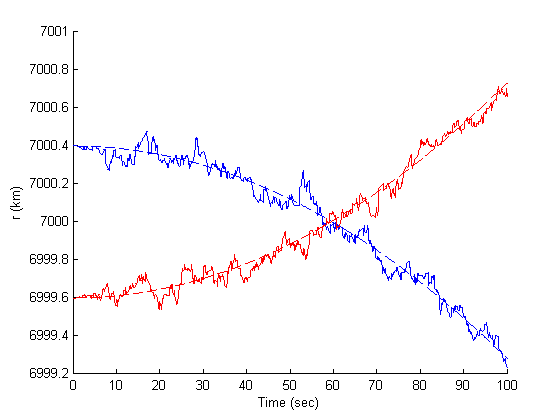
\includegraphics[width=9cm]{EKF.png}\hspace*{0.07\textwidth}}
	}
\centerline{
	\subfigure[JPDAF]{\hspace*{0.07\textwidth}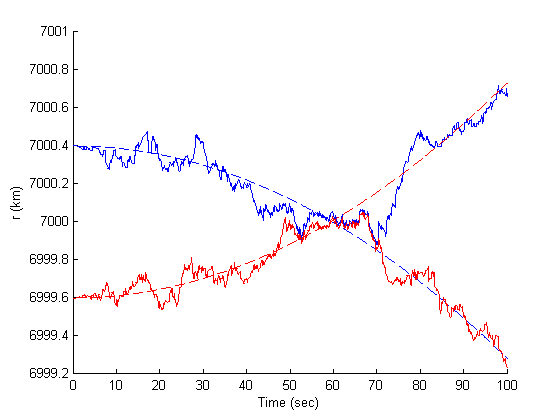
\includegraphics[width=9cm]{JPDAF.png}\hspace*{0.07\textwidth}}
	}
\centerline{
	\subfigure[C-JPDAF]{\hspace*{0.07\textwidth}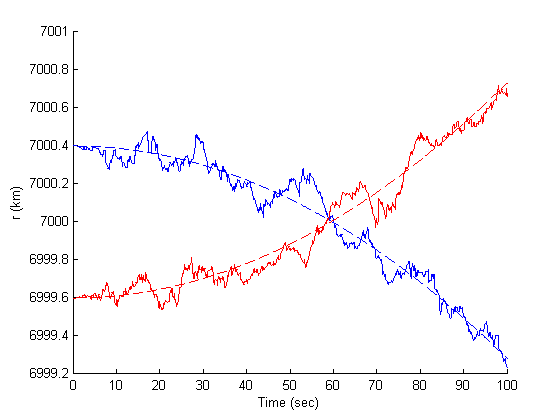
\includegraphics[width=9cm]{CAOJPDAF.png}\hspace*{0.05\textwidth}}
	}
\caption{Target 1 is represented in blue and target 2 is represented in red. A solid line represents an estimate and a dotted line represents the truth. The JPDAF is subject to coalescence of the neighboring track, causing the estimations to switch trajectories. The C-JPDAF is subject to much less coalescence and hence does not exhibit this problem.}
\label{AllAlgorithms}
\end{figure}

The corresponding results for each of  EKF, JPDAF, and C-JPDAF algorithms are illustrated in Figure \ref{AllAlgorithms}. 
First, EKF exhibits good estimation performance as there is no error or uncertainty in data association. The performance of JPDA is similar to EKF when two satellites are far apart from each other. However, when $50\leq t\leq 70$ seconds, two satellites become closer, and the estimated states are coalesced. When $t\geq 70$ seconds, the estimated states are incorrectly crossed. This illustrates undesirable performance of JPDAF especially for crossing targets. 

The proposed C-JPDAF does not exhibit the incorrect, crossed estimation of JPDA, and the estimated states follows each of the correct trajectories throughout the crossing orbital trajectories. The resulting RMS errors for the orbital radius of each method are summarized at Table \ref{tab:RMS}. This illustrates that the performance of the proposed C-JPDAF is comparable to EKF where there is no error in data association. 

\begin{table}
\caption{Estimation results}\label{tab:RMS}
\centerline{
\begin{tabular}{ccc}\hline
Method & Radial RMS Error (km) & Computation time (sec) \\\hline
EKF & 1.438e-05 &6.118\\
JPDAF & 7.1242e-05 &6.130\\
C-JPDAF & 2.3145e-05  & 19.864 \\\hline
\end{tabular}}
\end{table}

The major drawback of the C-JPDAF is the added computation time. However, the results of all three simulated algorithms (EKF, JPDAF, and C-JPDAF) are nearly identical when the estimates are not near the crossing region. Hence, the C-JPDAF can be turned on only during these close proximity regions, then turned off when unnecessary to improve the computational efficiency. 


%First, JPDAF is unable to maintain the correct trajectories of the estimates because the tracks coalesce so much that %correctly labeling the estimates becomes very difficult; when measurements from either target are sufficiently spread after the crossing, the JPDAF decision of trajectories that the estimates follow becomes ambiguous as the estimates become ambiguous. 

%Secondly, within $20 sec$ of crossing ($201$ measurements), the number of incorrect associated (weighted less than $50\%$ likelihood of association) for the JPDAF was $92$ whereas for the C-JPDAF this number was $70$. Comparing the performance of all three algorithms, the radial RMS error in the same window was calculated for the EKF as $1.4425\times10^{-05} km$, for the JPDAF $2.3014\times10^{-05} km$, and for the C-JPDAF $2.3858\times10^{-05} km$. This metric demonstrates the uncertainty of association degrades the estimates as the EKF performs significantly better than algorithms where measurement origination is unknown. The JPDAF is performs slightly better than the C-JPDAF with this metric, but this is a small drawback when compared with the ability to maintain correct tracks after crossing. The largest drawback of the C-JPDAF is the computational cost; running the simulations on the same computer, the JPDAF only required $7.518sec$ to run the program whereas the C-JPDAF required $25.785sec$ to run.

%_______________________________________________%

\section{Conclusions and Future Work}
\label{ConclusionFutureWork}
We explore a new approach to reduce coalescence of close proximity multi-target tracking. The estimator gains are chosen such that a weighted cost with respect to posterior uncertainty and similarity is minimized. The proximity similarity portion of the Matusita's measure is chosen to evaluate the similarity. Necessary conditions for optimality are derived, and they are solved numerically to obtain optimal estimator gains. Numerical examples illustrate that it exhibits excellent estimation and data association properties for crossing tracks in close proximity. Compared with other techniques to avoid coalescence, the proposed approach has simpler structures. Future works include generalizing C-JPDAF for arbitrary number of targets with clutter, and improving the computational efficiencies. 

%We take the derivative of the similarity cost for both estimates, yielding a result with no closed form solution, but involving expressions with low computational cost that can be solved with a nonlinear equation solver. In practice, a small similarity cost relative to the uncertainty cost yields best results; hence, the algorithm requires less time if the initial guesses of the Kalman gains are chosen.


%We validate the theory with numerical simulations. The C-JPDAF shares measurements in the same way as the JPDAF, but the tracks tend to maintain separation; the C-JPDAF does not prevent the estimates from crossing as the targets in the trajectory are designed to do. The major drawback of the C-JPDAF is the added computation. However, the results of all three simulated algorithms (EKF, JPDAF, and C-JPDAF) are nearly identical when the estimates are not near the crossing region (even if on the wrong trajectory). Hence, the C-JPDAF can be turned on only during these close proximity regions, then turned off when unnecessary to be replaced by a less computationally expensive algorithm.

%The C-JPDAF can be extended to a variety of multi-target tracking applications when targets share measurements due to close proximity. One example, very close to that presented in Section \ref{NumRes}, is keeping logs of satellites using phased-array radar systems. In cases where satellites have similar measurement predictions over long periods of time, satellite tracking becomes much more difficult. Implementing a simple JPDAF can serve to coalesce the estimates, which can cause the estimates of the satellites to switch trajectories as shown in this paper. Therefore, including the C-JPDAF under certain proximity conditions can expand our ability to track satellites. The C-JPDAF has tracking applications for space, aerial, and underwater vehicles in close proximity and identification of individual agents in multi-agent systems.

%Much like the Kalman filter, the C-JPDAF can be effective for systems with well-known Gaussian distributions of state, sensor noise, and process. This paper has assumed that measurements come from a single target of interest at a single time and not clutter. Future work may involve expanding the capabilities of the algorithm. We can consider the measurements as a scan, or so that multiple measurements, including those from external sources of clutter, may belong to multiple targets at any time step as a JPDAF does without the assumptions of this paper. A general form of this algorithm could be derived for these conditions. Furthermore we can explore other techniques to measure similarity. By only using the proximity portion Matusita's measure, we are assuming the covariances of the estimates are close, which is not always accurate in all applications, and another future direction of this work.


\begin{appendix}
\label{append}

\subsection{Proofs}

\paragraph{Derivation of the Association Probability}
The association probability at time step $k$ (this subscript will be omitted from this appendix) is given as follows from~\cite[Section 9.3]{TrackDataAssoc}
\begin{align}
\label{beta_all_terms}
\beta_i\equiv P(\Theta_i|z)=&\frac{1}{c}\frac{\phi!}{V}\displaystyle\prod_{j=1}^{m_k} f_{i_j}^{\tau_j}\displaystyle\prod_{i=1}^{T} P(\Theta_i)^{\delta_i}(1-P(\Theta_i))^{1-\delta_i}
\end{align}
where $c$ denotes a normalizing constant, $\phi$ denotes the number of unassociated measurements, $\delta$ denotes the binary target detection indicator, $V$ denotes an arbitrary volume that all targets fall inside, $j$ denotes an individual meausurement in a single update, $m_k$ denotes the total number of measurements that may be associated with a target, $f_{i}$ is the Gaussian pdf of target $i$, $\tau$ denotes the measurement association indicator, $T$ denotes the total number of targets, and $P(\Theta_i)$ denotes the probability of detecting target $i$.
We incorporate all of the assumptions from Section \ref{DAP} to simplify the weighting term for the estimates.
Let ${\bf{\Theta}}\in[\Theta_1, \Theta_2]$, as both possible outcomes, namely that target $1$ is measured or target $2$ is measured.
Each estimate may receive at most a single measurement, so $m_k=1$.
Because all events ${\bf{\Theta}}$ fall inside an arbitrary volume $V$, or are subject to being measured, the measurement association indicator $\tau=1$, meaning that measurement $k$ is associated with exactly one of the two targets.
Hence, the number of unassociated measurements $\phi({\bf{\Theta}})=0$ because the event that neither target is measured $\Theta_0\notin{\bf{\Theta}}$.
The binary target detection indicator is defined as $\delta_i(\Theta_i)=1$ if measurement $k$ is associated with target $i$ and $\delta_i(\Theta_i)=0$ otherwise.
The detection probabilities are generalized to $y$ estimates such that $P(\Theta_i)=\frac{1}{y}$ for equal likelihood of event $\Theta_i$.
Therefore, Equation \ref{beta_all_terms} reduces to
\begin{align}
\beta_i=&\frac{1}{cV}f_{i}\frac{1}{y}(1-\frac1y)^{T-1}.
\end{align}
Solving for $c$,
\begin{align}
c=&\frac{1}{V}\frac{1}{y}(1-\frac1y)^{T-1}\displaystyle\sum\limits_{l=1}^y f_{l}.
\end{align}
Hence, the simplified weighting considering the assumptions of this paper is
\begin{align}
\beta_i=\frac{f_i}{\displaystyle\sum\limits_{l=1}^y f_{l}}
\end{align}
which is equivalent to Equation \ref{eqn:betaik} for two estimates.


\paragraph{Derivation of Posteriori Covariance}

The second proof shows how the measurement updates may take a more manipulatable form under the assumptions. From~\cite[Section 6.4]{TrackDataAssoc},
\begin{align}
\bar e=&\displaystyle\sum\limits_{i=1}^{m_k}\beta_ie_i=\beta_ie_i\\
\hat x^+_i=&\hat x^-_i+K_i\bar e=\hat x^-_i+\beta_iK_ie_i.
\end{align}
Because only one innovation is calculated per target, there is no spread in the innovations term on each target, so this portion of the covariance $\tilde{P}=0$, which would normally be included in the JDPAF without these assumptions. The posterior covariance of target $i$ conditioned on event $\Theta_i$ is defined for any $K_i$ from ~\cite[Section 4.2]{OptEst1}:
\begin{align}
\begin{split}
P_{i}^C=&(I-K_{i}H_{i})P_{i}^{-}(I-K_{i}H_{i})^T+K_{i}R_{i}K_{i}^T\\
=&P^--K_{i}H_{i}P_{i}^{-}-P_{i}^{-}H_{i}^TK_{i}^T\\
&+K_{i}(H_{i}P_{i}^{-}H_{i}^T+R_i)K_{i}^T.
\end{split}
\end{align}
Let $\beta_{0_i}$ be the probability that target $i$ is not measured; with only one measurement considered each time step; hence, $\beta_{0_i}=1-\beta_i$. Again from~\cite[Section 6.4]{TrackDataAssoc},
\begin{align}
\begin{split}
P^+_i=&\beta_{0_i}P^-_i+(1-\beta_{0_i})P_i^C+\tilde{P}\\
=&(1-\beta_i)P^-+\beta_i[P^--K_{i}H_{i}P_{i}^{-}\\
&-P_{i}^{-}H_{i}^TK_{i}^T+K_{i}(H_{i}P_{i}^{-}H_{i}^T+R_i)K_{i}^T]\\
=&P^-_i-\beta_i[K_{i}H_{i}P_{i}^{-}+P_{i}^{-}H_{i}^TK_{i}^T\\
&-K_{i}(H_{i}P_{i}^{-}H_{i}^T+R_i)K_{i}^T].
\end{split}
\end{align}

\end{appendix}


\bibliography{BibMaster}
\bibliographystyle{IEEEtran}



\end{document}


%A considerable amount of work has been done to solve the data association problem. Approaches vary in their performance, including the portion of correct associations, the ability to maintain the correct tracks, and the computational cost. In this section, we examine some of the current techniques with respect to tracking two objects in close proximity and propose a new approach to solve this problem.
%
%The multiple hypothesis tracking (MHT) approach considers multiple hypotheses for how the data may be associated for multiple tracks~\cite{MHT1}. As new information becomes available, hypotheses are evaluated, in some cases removed, and predicted again. However in complicated problems, the number hypothesis may explode. One approach to remove this issue from the close proximity problem is known as track pruning, where incompatible tracks are highlighted and only the most likely tracks are considered. This approach is complex and involves a high computational cost, so implementing this approach in real-time is very difficult. Furthermore according to~\cite{PHD1}, MHT is subject to poor results with objects in close proximity.
%
%The probability hypothesis density (PHD) process is a propagation of the first moment of a joint distribution~\cite{PHD2}. A typical PHD considers a sub-area of interest where peaks from the integral of the PHD are considered objects. In many cases, the PHD filter is hindered by computational complexity, growing exponentially with the number of objects and further increasing when the possibility that objects may enter or leave the sub-area considered. An approach described in~\cite{PHD1} maintains a tracker for each object of interest. Each tracker accounts for a priori estimates of state and dynamics to predict the probability densities for the next time step. The process is complex and involves separating the sub-spaces into cells wherein likelihoods of each object are used to define peaks and dummy peaks, where a single track or multiple tracks exist, respectively. This approach can be more computationally expensive than other recursive approaches as the algorithm is among the most complex and the resolution (defined by size of the cells where peaks lie) will require modification as objects become close.
%
%The nearest neighbor filter (NNF) is a heuristic approach that calculates the magnitude between the measurement and its prediction~\cite{JPDAF1}; the state with smallest square Mahalanobis distance of the innovation and its covariance receives a filtered update with the measurement while all other states of interest are updated with only their predictions~\cite{NN2}; this is referred to as a \emph{hard decision}~\cite{JPDAF1}. This approach adds a simple step to the EKF at the cost of accuracy as the probability of association is not explicitly calculated.
%
%The JPDAF is an extension of the probabilistic data association filter (PDAF) described in~\cite{JPDAF1} and~\cite{TrackDataAssoc}, which calculates the probabilities that measurements belong to an individual estimate. The JPDAF is designed to track multiple objects of interest. The estimates are updated with a \emph{soft decision}, or by a weighting factor based from the probability of association. However, when more than one object of interest share measurements, the objects are subject to a measurement updates that draw the estimates together, or coalesce the estimates.
%
%There are a few approaches to remove coalescence from the JPDAF. Much like the MHT, some approaches iinvolve track pruning and are detailed in~\cite{Coal1},~\cite{Coal2},~\cite{Coal_d}, and~\cite{Coal_e}, but this is computationally complex and can suffer when implementing the approach recursively. Other techniques such as those described in~\cite{Coal_c},~\cite{Coal_g},~\cite{Coal_i}, and~\cite{Coal_j} involve assigning hard decisions. The criteria and performance of these techniques vary, but each eliminate coalescence by never sharing a measurement, which can yield fully weighted incorrect associations that may cause detrimental effects such as estimates switching trajectories of crossing tracks. To decrease this problem, an arbitrary scaling factor is applied in~\cite{Coal_f} wherein the more likely association is given more weight as the less likely association weightings are decreased, yielding a hybrid technique between the NNF and the JPDAF. This approach may yield improved results with a heuristic weighting scheme but results vary with the application and expected data.
%
%Therefore, we propose a systematic approach that minimizes a weighted cost of uncertainty and similarity. We design the KMMJPDAF to minimize the posterior uncertainty much like the Kalman filter in addition to evaluating the Mahalanobis distance involved with updating the states. The paper is organized as follows: the problem is formally presented in Section \ref{ProbDef}. The optimal gain derivation and algorithm description is presented in Section \ref{KMM}. We discuss how to implement the algorithm and how to appropriately weight the minimized cost function in section \ref{AlgImpTuning}. We consider a satellite tracking example of this technique in Section \ref{NumRes}. Finally, we discuss results and applications for the KMMJPDAF in Section \ref{ConclusionFutureWork}.







%\section{Problem Definition}
%\label{ProbDef}
%The objects of interest are assumed to have nonlinear dynamics and each have Gaussian distributed estimates. We evaluate objects at time $k$ and linearize the system dynamics with respect to time $k-1$. We define the JPDAF algorithm such that we update the state as measurements are received, i.e. we only consider a single measurement rather than a scan of measurements. Furthermore, this research is concerned with the two estimates in very close proximity; hence we assume that the measurement originations are from a single object of interest and not from other sources of clutter.
%
%\subsection{Time Update} We denote an estimate of state with a $\hat{.}$, and the estimates before and after the measurement update with a $.^-$ and $.^+$, respectively. We define $x\in \Re^{n\times1}$ as the state vector and $P\in\Re^{n\times n}$ as its covariance. The time update provides the predicted state and covariance
%\begin{gather}
%\hat{x}_{k}^{-}=A_{k-1}\hat{x}_{k-1} \\
%P_{k}^{-}=A_{k-1}P_{k-1}A_{k-1}^T+Q_k.
%\end{gather}
%The covariance of process noise is captured in $Q_k$ and no control input is considered.
%
%\subsection{Measurement Update} The measurement update requires an innovation
%\begin{equation}
%\label{innovation}
%e_{k}=z_{k}-\hat z_{k|k-1}
%\end{equation}
%where $z_{k}\in\Re^{m\times1}$ is the measurement received and measurement prediction $\hat z_{k|k-1}=H_{k}\hat{x}_{k}^{-}$; $H_{k}$ maps $\hat{x}_{k}^{-}$ from the state space to the measurement space.% Check this line terminology
%We simplify the equations for probability of association from~\cite{JPDAF1} and~\cite{TrackDataAssoc} to include only a single measurement that always belongs to either one of the two objects considered; hence the process of association is limited two mutually exclusive scenarios: we measure object 1 and not object 2 or we measure object 2 and not object 1. After some manipulation we can show for object $t$, the relative probability $\beta_t$ is simplified to
%\begin{gather}
%\beta_t=\frac{f_t}{\displaystyle\sum\limits_{\tau=1}^2 f_{\tau}} \\
%f_t=\mathcal{N}[z_{k};\hat z_{k|k-1},S].
%\end{gather}
%The innovation covariance $S$ is defined as
%\begin{equation}
%S_k=H_{k}P_{k}^{-}H_{k}^T+R_k
%\end{equation}
%where $R_k$ is the covariance of the measurement. The gain to minimize the posterior uncertainty with cost function $J_P=\tr{P_{k+1}^{+}}$ is equivalent to the Kalman gain
%\begin{equation}
%\label{KalmanGain}
%K_{k}=P_{k}^{-}H_{k}^TS_k^{-1}
%\end{equation}
%which is used to calculate the updated state and its covariance for each estimate
%\begin{gather}
%\label{xhatp}
%\hat{x}_{k}^{+}=\hat{x}_{k}^{-}+\beta K_{k}e_{k} \\
%\label{oldPp}
%P_{k}^{+}=P^-_{k}-\beta K_{k}S_kK_{k}^{T}
%\end{gather}
%for the JPDAF, but not for the KMMJPDAF. For the KMMJPDAF we derive a new gain which is not compatible with Equation \ref{oldPp}, which is a manipulation involving Equation \ref{KalmanGain} of the original form (ignoring the $\beta$ term)
%\begin{equation}
%\label{genPp}
%P_{k}^{+}=(I-K_{k}H_{k})P_{k}^{-}(I-K_{k}H_{k})^T+K_{k}R_kK_{k}^T
%\end{equation}
%from ~\cite{OptEst1}. Hence in order to properly update the posterior covariance when we include coalescence into the minimization, we manipulate Equation \ref{genPp} to involve relative weighting $\beta$ of the measurement update. Note that time step subscripts will be assumed at $k$ from here forward for simplicity. Obtaining a gain accounting for posterior uncertainty and coalescence takes the generalized form
%\begin{equation}
%\label{newPp}
%P^+=P^--\beta[KHP^-+P^-H^TK^T-K(HP^-H^T+R)K^T].
%\end{equation}
%Note that if we insert the Kalman gain from Equation \ref{KalmanGain} into Equation \ref{newPp}, we can manipulate the result to Equation \ref{oldPp}.

%\subsection{Uncertainty Cost} The derivation of $J_P$ is a fairly straightforward adaptation of the Kalman filter from~\cite{OptEst1} with the included JPDAF weighting. Evaluating the trace of Equation \ref{newPp} for object 1,
%\begin{align}
%\begin{split}
%J_{P,1}=&\tr{P_1^+} \\
%=& \tr{P_1^-}+\beta_1(\tr{K_1(H_1P_1^-H_1^T+R_1)K_1^T}\\
%&-2\tr{K_1H_1P_1^-}).
%\end{split}
%\end{align}
%We can take its derivative $\frac{\partial J_{P,1}}{\partial K_{1}}$ using the property $\frac{\partial}{\partial X}\tr{XYX^T}=2XY$ for symmetric $Y$ to obtain
%\begin{align}
%\label{CostP}
%\begin{split}
%\frac{\partial J_{P,1}}{\partial K_{1}}&=2\beta_1\{{K_1(H_1P_1^-H_1^T+R_1)-P_1^-H_1^T}\}.
%\end{split}
%\end{align}
%
% \subsection{Similarity Cost} We choose the Mahalanobis distance to measure similarity because it yields a scalar result and taking its derivative with respect to measurement update gains is possible. We use $P_1^-$ as the covariace estimation of object 1 for the Mahalanobis distance with respect to the estimated mean of object $2$ can take the form
%\begin{align}
%\label{M1}
%M_1=u_1^{\frac{1}{2}}
%\end{align}
%where
%\begin{align} \label{u_1}
%\begin{split}
%u_1=&(\hat x_1^+-\hat x_2^+)^{T}{P_1^-}^{-1}(\hat x_1^+-\hat x_2^+)\\
%=&\{\hat x_1^{-T}{P_1^-}^{-1}\hat x_1^-
%-2\hat x_1^{-T}{P_1^-}^{-1}\hat x_2^-\\
%&+2\beta_1(\hat x_1^{-}-\hat x_2^{-})^T{P_1^-}^{-1}K_1e_1
%+\hat x_2^{-T}{P_1^-}^{-1}\hat x_2^-\\
%&+2\beta_2(\hat x_2^{-}-\hat x_1^{-})^T{P_1^-}^{-1}K_2e_2
%+\beta_1^2e_1^TK_1^T{P_1^-}^{-1}K_1e_1\\
%&-2\beta_1\beta_2e_2^TK_2^T{P_1^-}^{-1}K_1e_1+\beta_2^2e_2^TK_2^T{P_1^-}^{-1}K_2e_2\}
%\end{split}
%\end{align}
%which is the most reduced form to differentiate with respect to $K_1$ and $K_2$. However, the Mahalanobis distance is an increasing measure as similarity decreases. Therefore we wish to minimize $M_1^{-2a}$ for $a>0$. Furthermore as the Mahalanobis distance is a scalar quantity, we can use the property $\frac{\partial g(u_1)}{\partial K_1}=\frac{\partial g(u_1)}{\partial u_1}\frac{\partial u_1}{\partial K_1}$ such that $J_{C,1}=M_1^{-2a}=g(u_1)=u_1^{-a}$. We take the derivative of the similarity measure using $u_1=f(K_1,K_2)$ from Equations \ref{M1} and \ref{u_1} as well as the properties $\frac{\partial}{\partial X} \tr{AXB}=A^TB^T$ and $\frac{\partial}{\partial X}\tr{AXBX^TC}=A^TC^TXB^T+CAXB$ to obtain, after some manipulation,
%\begin{align}
%\begin{split}
%\label{CostS}
%\frac{\partial J_{S,1}}{\partial K_1}=&-au_1^{-(a+1)}\frac{\partial u}{\partial K_1}\\
%=&2a\beta_1u_1^{-(a+1)}\{
%{P_1^-}^{-1}(\hat x_2^--\hat x_1^-)\\
%&-\beta_1{P_1^-}^{-1}K_1e_1
%+\beta_2{P_1^-}^{-1}K_2e_2
%\}e_1^T.
%\end{split}
%\end{align}
%
%We absorb the constants from Equations \ref{CostP} and \ref{CostS} into $c$ from Equation \ref{CostDef} and use a nonlinear equation solver for the optimal gains $K_1$ and $K_2$ in the joint equations
%\begin{align}
%\label{Opt1}
%\begin{split}
%\frac{\partial J_{1}}{\partial K_{1}}=&K_1(H_1P_1^-H_1^T+R_1)-P_1^-H_1^T\\
%&+cu_1^{-(a+1)}\{
%{P_1^-}^{-1}(\hat x_2^--\hat x_1^-)\\
%&-\beta_1{P_1^-}^{-1}K_1e_1
%+\beta_2{P_1^-}^{-1}K_2e_2
%\}e_1^T\\
%=&0_{n\times m}
%\end{split}
%\end{align}
%and similarly
%\begin{align}
%\label{Opt2}
%\begin{split}
%\frac{\partial J_{2}}{\partial K_{2}}=&K_2(H_2P_2^-H_2^T+R_2)-P_2^-H_2^T\\
%&+cu_2^{-(a+1)}\{
%{P_2^-}^{-1}(\hat x_1^--\hat x_2^-)\\
%&-\beta_2{P_2^-}^{-1}K_2e_2
%+\beta_1{P_2^-}^{-1}K_1e_1
%\}e_2^T\\
%=&0_{n\times m}.
%\end{split}
%\end{align}
%These equations vary in computational cost depending on the level of precision of the nonlinear equation solver. Note that ${P_1^-}^{-1}$ and ${P_2^-}^{-1}$ are symmetric inverses and must only be calculated once each.


%\section{Algorithm Implementation and Tuning}
%\label{AlgImpTuning}
%This algorithm requires considerably more computational cost than the JPDAF alone; hence, we only implement this algorithm when the likelihood of coalescence is high. For example, if the association of a measurement belongs primarily to a single estimate, the KMMJPDAF and JPDAF yield similar results so we choose JPDAF because of its closed form solution and hence lower computational cost. Therefore depending on the application, we determine thresholds such that beyond some spacing between the a priori estimates we default to the JPDAF algorithm for speed.
%
%We must also examine the shape of the cost function. Consider Figure \ref{CostTrends}, which contains a variation of a single element of $K_1$ from an example in Section \ref{NumRes} and plots both cost functions of object 1. The uncertainty cost minimizes at a single point. However, the similarity cost contains a maximum. If we incorrectly choose $K_1$ and $K_2$ to maximize $J_S$, this would serve to increase coalescence because similarity would be increasing at a maximum rate due only to a measurement update.
%
%\begin{figure}
%\centerline{
%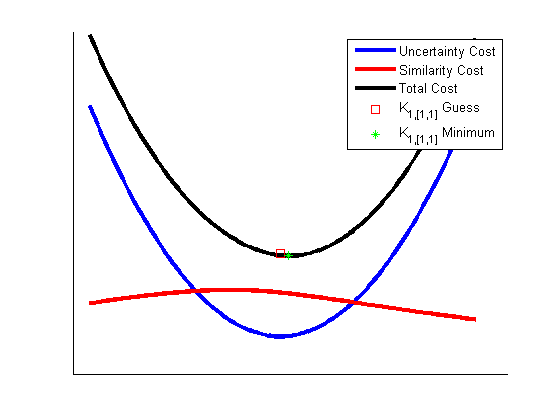
\includegraphics[width=9cm]{CostTrends.png}
%	}
%\caption{The cost functions of object 1 ($J_{P,1}$, $cJ_{C,1}$, and $J_{1}$) are examined under the variation of a single element of $K_1$. The resulting cost function (black) is minimized slightly to the left of the uncertainty cost function (blue). In Kalman filtering applications, including the JPDAF, only the uncertainty cost function is minimized.}
%\label{CostTrends}
%\end{figure}
%
%There are a few approaches to avoid this detrimental scenario. First, we can choose $a$ and $c$ properly. Decreasing $a$ serves to amplify and flatten out $J_S$. Once a desired cost function shape as achieved, we can choose $c$ to bring $J_S$ to an appropriate scaling. In practice, the JPDAF is a very effective algorithm for estimation of multiple objects, which only relies on $J_P$, so $J_S$ is chosen to be very small in comparison only to remove coalescence from the estimates (Figure \ref{CostTrends} shows $cJ_{S,1}$ much larger in magnitude than in practice for illustration). Choice of these parameters leads to trade-offs: if $a$ is decreased along with $c$, the similarity cost varies less, decreasing the beneficial effects of the KMMJPDAF over the JPDAF. However, when $a$ is increased (and $c$ is increased to compensate), we may incorrectly solve for the similarity maximizing point.
%
%We explore two techniques to find an effective minimization. First, we choose the initial guess of $K_1$ and $K_2$ to be that of the EKF, which is already located near the minimized point of uncertainty. Secondly, we only implement the KMMJPDAF when the a priori estimates are sufficiently spaced apart. This way we can maintain the desirable shape of the cost function and implement the KMMJPDAF for the majority of the region where coalescence poses an issue. Therefore, we have both minimum and maximum estimate spacing thresholds for which KMMJPDAF is appropriate.

%In fact, the results are very similar with two noteworthy differences. The first is that within $20 sec$ of crossing ($201$ measurements), the number of incorrect associated (weighted less than $50\%$ likelihood of association) for the JPDAF was $64$ whereas for the KMMJPDAF the number was $58$, but this is a minor difference in the metric. The second difference is that the JPDAF completed in $4.212sec$ while the KMMJPDAF ran in $6.8952sec$ on the same computer. For real-time implementation, either algorithm is capable of receiving these simple range measurements as described above, but when measurements are more complicated or are received at a faster rate, there can be cases where the performance of the JPDAF computational time makes the KMMJPDAF an inferior algorithm.
%
%The noise of the measurements are increased in second example (Figure \ref{Case2}), and this causes the JPDAF to permanently lose the correct association after the crossing. The optimization of the KMMJPDAF compensates for the coalescence of the tracks, and hence correct track maintenance is achieved properly with this algorithm. The result of this example does not imply that the KMMJPDAF is impervious the the effects of coalescence; rather including similarity in the minimization serves to remove some of the coalescence from measurement updates. For the case presented here, choosing the KMMJPDAF rather than the JPDAF increases the computational time from $4.1964sec$ to $6.8018sec$ to maintain the estimates with the correct trajectories.
%
%We now use the last example to demonstrate the importance of choosing the parameters correctly for the effective implementation of the KMMJPDAF. In Figure \ref{changeParameters}.(a), we increase $a$ such that $a=1$, which serves to attenuate the similarity cost function. As a result, the gains are chosen to minimize uncertainty with greater weight much like the JPDAF. This results in increasing coalescence, yielding a poorer estimation of the states. In this case, the estimates are drawn very close together and diverge incorrectly.
%
%We consider the same example but this time increase $c$ such that $c=1\times10^{-7}$, shown in Figure \ref{changeParameters}.(b). Increasing $c$ increases the similarity cost function proportionally according to Equation \ref{CostDef}. Contrary to the last example, the gains are chosen to decrease similarity of the estimates so much that the measurement updates serve to separate the estimates when the estimates become close. We experience the opposite effect with increasing $c$ than increasing $a$, but choosing either parameter poorly can lead to estimates switching trajectories.
